\chapter{Conclusion}

\section{Future Work}

\subsection{Automatic Differention of Solids}

\begin{lstlisting}
julia> using DualNumbers

julia> f(x) = 2x+1
f (generic function with 1 method)

julia> f(Dual(1,1))
3 + 2du
\end{lstlisting}



\subsection{Ray Tracing and Marching}

\todo{leave this section, would be good to discuss angle-based polyhedra
and or deficits for these ops}

When we look at the natural world we observe the
propogation of light energy. Our eyes recieve this light energy in the form
of photons. The study of ray tracing seeks to mimic such behavior for
computer visualizations and simulations. 

\begin{figure}[h!]
  \centering
    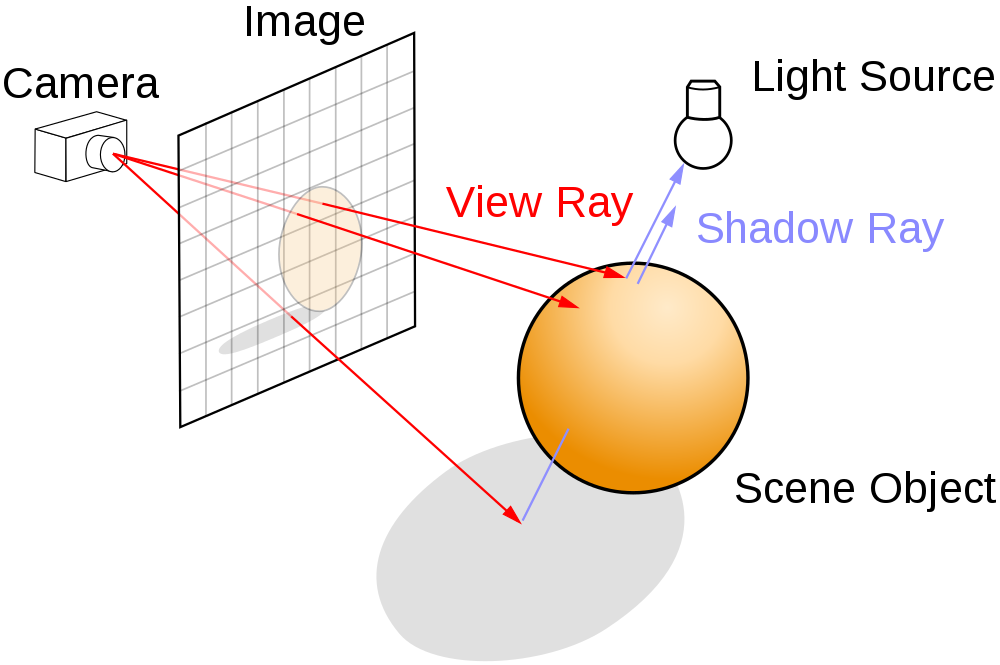
\includegraphics[width=0.75\textwidth]{img/ray_trace_diagram.png}
  \caption{An illustration of a Ray tracing.\protect\footnotemark}
  \label{fig:raytrace}
\end{figure}

\footnotetext{By Henrik (Own work) GFDL or CC BY-SA 4.0-3.0-2.5-2.0-1.0, via Wikimedia Commons}

Íñgo Quílez has done some of the most accessible work on real-time ray tracing.
His technique is called ray marching, and leverages the properties of functional
geometry.\cite{Quilez_2008}

\subsection{Engineering Solid Analysis}



